\documentclass[a4paper,12pt]{article}
\usepackage[T2A]{fontenc}    % кодировка
\usepackage[utf8]{inputenc}   % кодировка исходного текста
\usepackage{graphicx}
\usepackage{tikz}
\usepackage[english]{babel}
\addto\captionsenglish{\renewcommand{\figurename}{\textbf{Fig.}}}


%[english]{babel}  % локализация и переносы

%\usepackage[russian]{babel}

%\usepackage[T1,T2A]{fontenc}

\begin{document}

\section{THE DEVELOPMENT OF PARALLEL
         \begin{center}MACHINES\end{center}}
   As we have seen from the preceding section, the introduction of
parallelism into computer implementation occurred almost everywhere
where possible. And so there is no simple and single line of
development leading to modern parallel processing machines. Before
considering this development further, therefore, it is important to
recognize that many levels exist where parallelism may be used. Let us
summarize the main categories:

\begin{itemize}
  \item[i)] {\itshape Within functional units:} Arithmetic, logical
    and other operations can be implemented in bit-serial mode,
    parallel by bit groups, or on whole operands concurrently. Clearly
    there are limits to what can be done, and there is the question of
    cost and reliability of the extra hardware involved. However, this
    category does not generally affect the way in which a problem is
    formulated, although it does determine the speed of
    execution. Another area of parallelism in this category is the
    concurrent access to several interleaved memory units.

   \item[ii)] {\itshape Within processing elements:} At this level,
     the most obvious form of concurrency is between different
     operations executing in parallel on different operands. For this
     to be exploited, the problem formulation (the detailed machine
     coding in this case) needs to be appropriate to the PE
     organization. Another kind of concurrency is where there is only
     a single instruction at one time, but the functional unit to the
     instruction refers, for example a multiplier, may be able to
     process a stream of operands in an overlapped or pipelined
     fashion. Pipelining is a very powerful feature indeed, which we
     will discuss later. It can give significant improvements in
     execution speed even for simple sequences of entirely serial
     code.

   \item[iii)] {\itshape Within uniprocessing computers:} Even with
     only a single processor, there are many activities that can
     proceed concurrently. An obvious example already mentioned is
     memory access, and another is I/O. In some ways, the concurrent
     operation of input-output is just a detail of system
     organization, since it is a way of keeping the operational
     memory full (or to empty it); if main memory were big enough,
     many of the I/O problems would vanish. However, when several
     uniprocessors need to inter-communicate in order concurrently
     to execute different tasks of the same job, then parallel I/O
     or inter-memory communication is a vital requirement --- and a
     difficult problem to solve.

   \item[iv)] {\itshape Many-processor systems:} An obvious category
     of concurrency is where a computer system contains several
     (often many) processors, either sharing main memory or not, and
     inter-communicating by some means. In the most usual example,
     the separate processors are used to execute quite independent
     jobs. This is the well-known multi-processor architecture, and
     the concurrency here is used not to speed up the execution of
     individual jobs, but the global throughput of the whole system.
     \noindent Much more interesting from the standpoint of our discussion
     here is where the different processors are used either to
     execute separate cooperating tasks within a given job or where
     even separate code sequences within a given program are
     executed concurrently.
     \noindent There is a very great difference here between computers where
     all the processing elements are identical, and operate in lock
     step, and where they differ.
\end{itemize}

   The way in which all the different levels of con currency are
exploited differs from one category to another. In the case of
functional parallelism, it is necessary to structure the machine
code appropriately, and so the characteristics of any compiler used
are of paramount importance. At the other extreme, in
multi-processing systems, it is the operating system which does the
job of allocating resources among concurrently executing jobs and
between processing and I/O. In all other categories, of central
importance is the structure of the job itself and so the choice of
algorithms used becomes the significant issue. We shall return to
this most important question later.\par\medskip

%\righthyphenmin=4
   At the present time, several machines exist whose architecture and
implementation have been expressly chosen to provide massive
parallel-processing capability. We shall describe some of them
later. However, in the previous two decades, a number of earlier
computer systems were developed where concurrency was a central
feature in implementation, and where nearly all the basic ideas on
which modern machines are based were tried out. In these machines, it
is not always easy to separate out any one feature as being most
significant, since several levels of concurrency were often
implemented in the same system. Nevertheless, there were perhaps three
separate lines of development whose evolution has been more or less
distinct, namely pipelining, the use of many functional units within a
uniprocessor, and systems of many cooperating processors. And there is
one other category which might be mentioned separately, that of
special-purpose computing systems. Let us briefly consider these four
categories.

\subsection{Pipelining}
   In many computational processes, the total process can be made to
   take place in a number of discrete steps or segments. For example,
   the processing of an instruction might be segmented into the
   separate phases of fetching the instruction, decoding, calculating
   the operand addresses, fetching the operands and executing the
   instruction. In {\bfseries Fig.1} the difference is shown
   diagrammatically between some unsegmented process {\bfseries P} and
   the same process separated into four sequential segments. There is
   no reason why the total time {\bfseries T} for an unsegmented
   process {\bfseries P} should differ from the sum of the separate
   segment times $t_1 + t_2 + t_3 + t_4$. The idea of pipelining
   is simply that if all the segments {\bfseries S} are implemented by
   physically separate sub-units, then they can operate together, and
   several processes may proceed concurrently in an overlapped
   fashion. {\bfseries Fig.1(b)} represents thus a processing pipe in
   which there may be up to four concurrent processes {\bfseries P} at
   any given instant.

\begin{figure}[h]
  \centering
  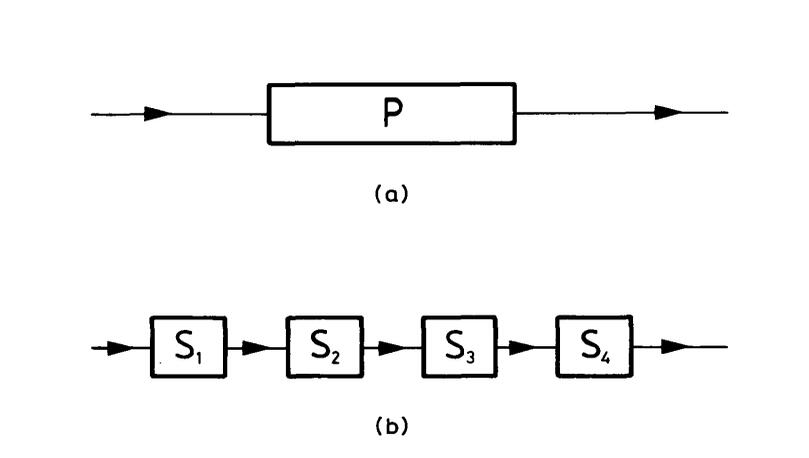
\includegraphics[width=0.75\textwidth]{figure_01}
  \caption{A process P in usegmented form (a) and suitable for
    pipelining (b)}
\end{figure}

   The advantage of a pipeline can be seen from \textbf{Fig.2} which
shows several processes P in concurrent execution. In the first
clock period only the first process is executing, but by clock
period 5 there are four processes of complete processes from a full
pipeline is one for every clock period, a potential improvement of
\textbf{m} compared with unsegmented processing, where \textbf{m} is the number of segments.
   
\begin{figure}[h]
  \centering
  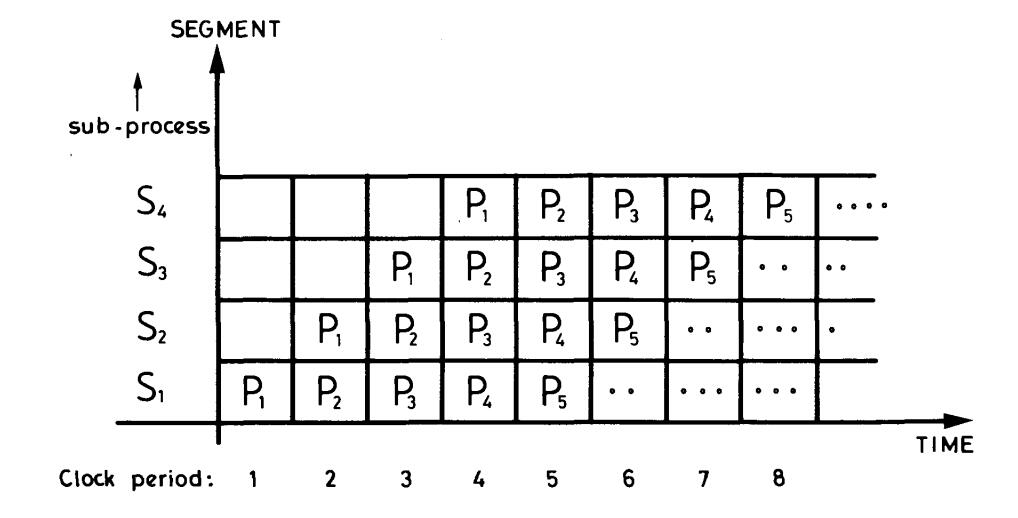
\includegraphics[width=0.75\textwidth]{figure_02}
  \caption{Timing diagram for a 4-segment pipeline}
\end{figure}

   The example above is that of pipelining in instruction processing,
and one of the earliest implementations of this idea
(in~rudimentary~form) was in the \textit{STRETCH} computer. But
pipelining can also be used with even greater effectiveness in
arithmetic processes. For example, a floating-point addition may be
segmented into, say, four execution phases: compare exponents,\\
normalize mantissa, add, normalize result. There is then in principle
no limit to the number of operands that can be processed in an
overlapped way at the maximum pipeline rate, an encouraging prospect,
bringing to mind the alliterative words of Alexander Pope:
\begin{quote}
  {\itshape ``And the smooth stream in smoother numbers flows''
    \begin{flushright} An Essay on Criticism \end{flushright}}
\end{quote}
   A machine which used pipelining in this fashion for instruction
processing was the Ferranti \textit{ATLAS} computer developed
jointly with Manchester University and first delivered in 1963. In
this machine, the floating-point addition time of 6 microseconds
for a single pair of operands, could be reduced to 1.6 microseconds
on average for a long stream.\medskip

   Pipelining has been employed at more than one level in machines,
and in different configurations. In the preceding examples the method
has been used either to overlap the processing of successive
instructions (in the I-unit) or the execution of successive operations
of the same kind on different operands (in a E-unit). Of course, one
can have both, and this was probably done for the first time in the
\textit{IBM 360/91} in the mid-sixties. However, a very interesting
application of pipelining of a somewhat different kind, also used in
the \textit{360/91}, is at the micro-system level, for example within a single
arithmetic operation. Here, for example in floating-point
multiplication or division, the function can be implemented as a
successive or iterative execution of a series of microfunctions; in
the case of multiplication, the microfunctions might be additions
(or~subtractions) of partial summands deriving from using one or more
bits of the multiplier. Then the same hardware segments are used
cyclically to process different parts of operands; but only one
instruction is being executed at any given time. So if, for example in
16-bit multiplications, 4-bit groups are being processed, one might
require four cycles through a pipeline of 5 segments to generate the
final product. Such a scheme is shown in \textbf{Fig.3}, where
\textbf{S} decodes each 4-bit group and provides 3 appropriately
scaled multiplicands to be summed (with proper signs) in a carry-save
adder \textbf{CSA-1}. In further cycles partial sums of accumulated
operands are added in \textbf{CSA-2} and \textbf{CSA-3}, but at the
last cycle (i.e. after 8 minor cycles) the final outputs of
\textbf{CSA-3} are summed in a carry-propagating adder \textbf{A} to
give a 32-bit product at the output.\medskip

% Перерисовать и добавить в виде схемы ---- !!!!!!!!!!!!!!!!!!!!!!
%\begin{figure}[h]
%  \centering
%  \includegraphics[width=0.75\textwidth]{figure_03}
%  \caption{An iterative pipeline multiplier}
%\end{figure}

\begin{figure}[h]
	\centering
	% Graphic for TeX using PGF
% Title: /home/ivasdtmbb/00_SPBPU_Politech_mycode/latex/Diagram1.dia
% Creator: Dia v0.97.3
% CreationDate: Fri Nov 10 14:13:05 2023
% For: ivasdtmbb
% \usepackage{tikz}
% The following commands are not supported in PSTricks at present
% We define them conditionally, so when they are implemented,
% this pgf file will use them.
\ifx\du\undefined
  \newlength{\du}
\fi
\setlength{\du}{15\unitlength}
\begin{tikzpicture}[even odd rule]
\pgftransformxscale{1.000000}
\pgftransformyscale{-1.000000}
\definecolor{dialinecolor}{rgb}{0.000000, 0.000000, 0.000000}
\pgfsetstrokecolor{dialinecolor}
\pgfsetstrokeopacity{1.000000}
\definecolor{diafillcolor}{rgb}{1.000000, 1.000000, 1.000000}
\pgfsetfillcolor{diafillcolor}
\pgfsetfillopacity{1.000000}
\pgfsetlinewidth{0.067101\du}
\pgfsetdash{}{0pt}
\pgfsetmiterjoin
\definecolor{diafillcolor}{rgb}{1.000000, 1.000000, 1.000000}
\pgfsetfillcolor{diafillcolor}
\pgfsetfillopacity{1.000000}
\fill (17.220095\du,-6.021956\du)--(30.472477\du,-6.021956\du)--(30.472477\du,-4.633495\du)--(17.220095\du,-4.633495\du)--cycle;
\definecolor{dialinecolor}{rgb}{0.000000, 0.000000, 0.000000}
\pgfsetstrokecolor{dialinecolor}
\pgfsetstrokeopacity{1.000000}
\draw (17.220095\du,-6.021956\du)--(30.472477\du,-6.021956\du)--(30.472477\du,-4.633495\du)--(17.220095\du,-4.633495\du)--cycle;
% setfont left to latex
% setfont left to latex
\definecolor{dialinecolor}{rgb}{0.000000, 0.000000, 0.000000}
\pgfsetstrokecolor{dialinecolor}
\pgfsetstrokeopacity{1.000000}
\definecolor{diafillcolor}{rgb}{0.000000, 0.000000, 0.000000}
\pgfsetfillcolor{diafillcolor}
\pgfsetfillopacity{1.000000}
\node[anchor=base,inner sep=0pt, outer sep=0pt,color=dialinecolor] at (23.846286\du,-5.119456\du){};
\pgfsetlinewidth{0.067101\du}
\pgfsetdash{}{0pt}
\pgfsetbuttcap
\definecolor{dialinecolor}{rgb}{0.000000, 0.000000, 0.000000}
\pgfsetstrokecolor{dialinecolor}
\pgfsetstrokeopacity{1.000000}
\draw (20.533191\du,-6.021956\du)--(20.533191\du,-4.633495\du);
\pgfsetlinewidth{0.067101\du}
\pgfsetdash{}{0pt}
\pgfsetbuttcap
\definecolor{dialinecolor}{rgb}{0.000000, 0.000000, 0.000000}
\pgfsetstrokecolor{dialinecolor}
\pgfsetstrokeopacity{1.000000}
\draw (23.846286\du,-6.021956\du)--(23.846286\du,-4.633495\du);
\pgfsetlinewidth{0.067101\du}
\pgfsetdash{}{0pt}
\pgfsetbuttcap
\definecolor{dialinecolor}{rgb}{0.000000, 0.000000, 0.000000}
\pgfsetstrokecolor{dialinecolor}
\pgfsetstrokeopacity{1.000000}
\draw (27.159382\du,-6.021956\du)--(27.159382\du,-4.633495\du);
\pgfsetlinewidth{0.067101\du}
\pgfsetdash{}{0pt}
\pgfsetbuttcap
\definecolor{dialinecolor}{rgb}{0.000000, 0.000000, 0.000000}
\pgfsetstrokecolor{dialinecolor}
\pgfsetstrokeopacity{1.000000}
\draw (27.787809\du,-4.621967\du)--(27.768720\du,-2.158482\du);
\pgfsetdash{}{0pt}
\pgfsetmiterjoin
\pgfsetbuttcap
\definecolor{diafillcolor}{rgb}{0.000000, 0.000000, 0.000000}
\pgfsetfillcolor{diafillcolor}
\pgfsetfillopacity{1.000000}
\fill (27.766596\du,-1.884453\du)--(27.601682\du,-2.251366\du)--(27.768720\du,-2.158482\du)--(27.937173\du,-2.248283\du)--cycle;
\definecolor{dialinecolor}{rgb}{0.000000, 0.000000, 0.000000}
\pgfsetstrokecolor{dialinecolor}
\pgfsetstrokeopacity{1.000000}
\draw (27.766596\du,-1.884453\du)--(27.601682\du,-2.251366\du)--(27.768720\du,-2.158482\du)--(27.937173\du,-2.248283\du)--cycle;
\pgfsetlinewidth{0.067101\du}
\pgfsetdash{}{0pt}
\pgfsetbuttcap
\definecolor{dialinecolor}{rgb}{0.000000, 0.000000, 0.000000}
\pgfsetstrokecolor{dialinecolor}
\pgfsetstrokeopacity{1.000000}
\draw (28.526631\du,-4.637835\du)--(28.551293\du,-2.166851\du);
\pgfsetdash{}{0pt}
\pgfsetmiterjoin
\pgfsetbuttcap
\definecolor{diafillcolor}{rgb}{0.000000, 0.000000, 0.000000}
\pgfsetfillcolor{diafillcolor}
\pgfsetfillopacity{1.000000}
\fill (28.554028\du,-1.892829\du)--(28.382639\du,-2.256206\du)--(28.551293\du,-2.166851\du)--(28.718123\du,-2.260177\du)--cycle;
\definecolor{dialinecolor}{rgb}{0.000000, 0.000000, 0.000000}
\pgfsetstrokecolor{dialinecolor}
\pgfsetstrokeopacity{1.000000}
\draw (28.554028\du,-1.892829\du)--(28.382639\du,-2.256206\du)--(28.551293\du,-2.166851\du)--(28.718123\du,-2.260177\du)--cycle;
\pgfsetlinewidth{0.067101\du}
\pgfsetdash{}{0pt}
\pgfsetbuttcap
\definecolor{dialinecolor}{rgb}{0.000000, 0.000000, 0.000000}
\pgfsetstrokecolor{dialinecolor}
\pgfsetstrokeopacity{1.000000}
\draw (29.208300\du,-4.629297\du)--(29.232962\du,-2.158313\du);
\pgfsetdash{}{0pt}
\pgfsetmiterjoin
\pgfsetbuttcap
\definecolor{diafillcolor}{rgb}{0.000000, 0.000000, 0.000000}
\pgfsetfillcolor{diafillcolor}
\pgfsetfillopacity{1.000000}
\fill (29.235697\du,-1.884291\du)--(29.064309\du,-2.247669\du)--(29.232962\du,-2.158313\du)--(29.399792\du,-2.251640\du)--cycle;
\definecolor{dialinecolor}{rgb}{0.000000, 0.000000, 0.000000}
\pgfsetstrokecolor{dialinecolor}
\pgfsetstrokeopacity{1.000000}
\draw (29.235697\du,-1.884291\du)--(29.064309\du,-2.247669\du)--(29.232962\du,-2.158313\du)--(29.399792\du,-2.251640\du)--cycle;
\pgfsetlinewidth{0.067101\du}
\pgfsetdash{}{0pt}
\pgfsetbuttcap
\definecolor{dialinecolor}{rgb}{0.000000, 0.000000, 0.000000}
\pgfsetstrokecolor{dialinecolor}
\pgfsetstrokeopacity{1.000000}
\draw (29.889970\du,-4.643980\du)--(29.914632\du,-2.172996\du);
\pgfsetdash{}{0pt}
\pgfsetmiterjoin
\pgfsetbuttcap
\definecolor{diafillcolor}{rgb}{0.000000, 0.000000, 0.000000}
\pgfsetfillcolor{diafillcolor}
\pgfsetfillopacity{1.000000}
\fill (29.917367\du,-1.898974\du)--(29.745978\du,-2.262351\du)--(29.914632\du,-2.172996\du)--(30.081462\du,-2.266322\du)--cycle;
\definecolor{dialinecolor}{rgb}{0.000000, 0.000000, 0.000000}
\pgfsetstrokecolor{dialinecolor}
\pgfsetstrokeopacity{1.000000}
\draw (29.917367\du,-1.898974\du)--(29.745978\du,-2.262351\du)--(29.914632\du,-2.172996\du)--(30.081462\du,-2.266322\du)--cycle;
\pgfsetlinewidth{0.067101\du}
\pgfsetdash{}{0pt}
\pgfsetmiterjoin
\definecolor{diafillcolor}{rgb}{1.000000, 1.000000, 1.000000}
\pgfsetfillcolor{diafillcolor}
\pgfsetfillopacity{1.000000}
\fill (27.229610\du,-1.786329\du)--(30.452803\du,-1.786329\du)--(30.452803\du,0.006703\du)--(27.229610\du,0.006703\du)--cycle;
\definecolor{dialinecolor}{rgb}{0.000000, 0.000000, 0.000000}
\pgfsetstrokecolor{dialinecolor}
\pgfsetstrokeopacity{1.000000}
\draw (27.229610\du,-1.786329\du)--(30.452803\du,-1.786329\du)--(30.452803\du,0.006703\du)--(27.229610\du,0.006703\du)--cycle;
% setfont left to latex
% setfont left to latex
\definecolor{dialinecolor}{rgb}{0.000000, 0.000000, 0.000000}
\pgfsetstrokecolor{dialinecolor}
\pgfsetstrokeopacity{1.000000}
\definecolor{diafillcolor}{rgb}{0.000000, 0.000000, 0.000000}
\pgfsetfillcolor{diafillcolor}
\pgfsetfillopacity{1.000000}
\node[anchor=base,inner sep=0pt, outer sep=0pt,color=dialinecolor] at (28.841207\du,-0.681544\du){};
\pgfsetlinewidth{0.067101\du}
\pgfsetdash{}{0pt}
\pgfsetbuttcap
\definecolor{dialinecolor}{rgb}{0.000000, 0.000000, 0.000000}
\pgfsetstrokecolor{dialinecolor}
\pgfsetstrokeopacity{1.000000}
\draw (27.800828\du,0.041317\du)--(27.807604\du,1.516386\du);
\pgfsetdash{}{0pt}
\pgfsetmiterjoin
\pgfsetbuttcap
\definecolor{diafillcolor}{rgb}{0.000000, 0.000000, 0.000000}
\pgfsetfillcolor{diafillcolor}
\pgfsetfillopacity{1.000000}
\fill (27.808863\du,1.790421\du)--(27.639435\du,1.425955\du)--(27.807604\du,1.516386\du)--(27.974934\du,1.424127\du)--cycle;
\definecolor{dialinecolor}{rgb}{0.000000, 0.000000, 0.000000}
\pgfsetstrokecolor{dialinecolor}
\pgfsetstrokeopacity{1.000000}
\draw (27.808863\du,1.790421\du)--(27.639435\du,1.425955\du)--(27.807604\du,1.516386\du)--(27.974934\du,1.424127\du)--cycle;
\pgfsetlinewidth{0.067101\du}
\pgfsetdash{}{0pt}
\pgfsetbuttcap
\definecolor{dialinecolor}{rgb}{0.000000, 0.000000, 0.000000}
\pgfsetstrokecolor{dialinecolor}
\pgfsetstrokeopacity{1.000000}
\draw (29.816618\du,0.028955\du)--(29.802510\du,1.505538\du);
\pgfsetdash{}{0pt}
\pgfsetmiterjoin
\pgfsetbuttcap
\definecolor{diafillcolor}{rgb}{0.000000, 0.000000, 0.000000}
\pgfsetfillcolor{diafillcolor}
\pgfsetfillopacity{1.000000}
\fill (29.799892\du,1.779562\du)--(29.635640\du,1.412296\du)--(29.802510\du,1.505538\du)--(29.971125\du,1.416098\du)--cycle;
\definecolor{dialinecolor}{rgb}{0.000000, 0.000000, 0.000000}
\pgfsetstrokecolor{dialinecolor}
\pgfsetstrokeopacity{1.000000}
\draw (29.799892\du,1.779562\du)--(29.635640\du,1.412296\du)--(29.802510\du,1.505538\du)--(29.971125\du,1.416098\du)--cycle;
\pgfsetlinewidth{0.067101\du}
\pgfsetdash{}{0pt}
\pgfsetbuttcap
\definecolor{dialinecolor}{rgb}{0.000000, 0.000000, 0.000000}
\pgfsetstrokecolor{dialinecolor}
\pgfsetstrokeopacity{1.000000}
\draw (28.841207\du,0.006703\du)--(28.853607\du,1.510965\du);
\pgfsetdash{}{0pt}
\pgfsetmiterjoin
\pgfsetbuttcap
\definecolor{diafillcolor}{rgb}{0.000000, 0.000000, 0.000000}
\pgfsetfillcolor{diafillcolor}
\pgfsetfillopacity{1.000000}
\fill (28.855866\du,1.784992\du)--(28.685109\du,1.421262\du)--(28.853607\du,1.510965\du)--(29.020599\du,1.417982\du)--cycle;
\definecolor{dialinecolor}{rgb}{0.000000, 0.000000, 0.000000}
\pgfsetstrokecolor{dialinecolor}
\pgfsetstrokeopacity{1.000000}
\draw (28.855866\du,1.784992\du)--(28.685109\du,1.421262\du)--(28.853607\du,1.510965\du)--(29.020599\du,1.417982\du)--cycle;
\pgfsetlinewidth{0.067101\du}
\pgfsetdash{}{0pt}
\pgfsetmiterjoin
\definecolor{diafillcolor}{rgb}{1.000000, 1.000000, 1.000000}
\pgfsetfillcolor{diafillcolor}
\pgfsetfillopacity{1.000000}
\fill (27.227410\du,1.887707\du)--(30.450602\du,1.887707\du)--(30.450602\du,3.680739\du)--(27.227410\du,3.680739\du)--cycle;
\definecolor{dialinecolor}{rgb}{0.000000, 0.000000, 0.000000}
\pgfsetstrokecolor{dialinecolor}
\pgfsetstrokeopacity{1.000000}
\draw (27.227410\du,1.887707\du)--(30.450602\du,1.887707\du)--(30.450602\du,3.680739\du)--(27.227410\du,3.680739\du)--cycle;
% setfont left to latex
% setfont left to latex
\definecolor{dialinecolor}{rgb}{0.000000, 0.000000, 0.000000}
\pgfsetstrokecolor{dialinecolor}
\pgfsetstrokeopacity{1.000000}
\definecolor{diafillcolor}{rgb}{0.000000, 0.000000, 0.000000}
\pgfsetfillcolor{diafillcolor}
\pgfsetfillopacity{1.000000}
\node[anchor=base,inner sep=0pt, outer sep=0pt,color=dialinecolor] at (28.839006\du,2.992492\du){};
\pgfsetlinewidth{0.067101\du}
\pgfsetdash{}{0pt}
\pgfsetbuttcap
\definecolor{dialinecolor}{rgb}{0.000000, 0.000000, 0.000000}
\pgfsetstrokecolor{dialinecolor}
\pgfsetstrokeopacity{1.000000}
\draw (29.833534\du,3.681929\du)--(29.829389\du,5.203465\du);
\pgfsetdash{}{0pt}
\pgfsetmiterjoin
\pgfsetbuttcap
\definecolor{diafillcolor}{rgb}{0.000000, 0.000000, 0.000000}
\pgfsetfillcolor{diafillcolor}
\pgfsetfillopacity{1.000000}
\fill (29.828643\du,5.477502\du)--(29.661887\du,5.111577\du)--(29.829389\du,5.203465\du)--(29.997389\du,5.112661\du)--cycle;
\definecolor{dialinecolor}{rgb}{0.000000, 0.000000, 0.000000}
\pgfsetstrokecolor{dialinecolor}
\pgfsetstrokeopacity{1.000000}
\draw (29.828643\du,5.477502\du)--(29.661887\du,5.111577\du)--(29.829389\du,5.203465\du)--(29.997389\du,5.112661\du)--cycle;
\pgfsetlinewidth{0.067101\du}
\pgfsetdash{}{0pt}
\pgfsetbuttcap
\definecolor{dialinecolor}{rgb}{0.000000, 0.000000, 0.000000}
\pgfsetstrokecolor{dialinecolor}
\pgfsetstrokeopacity{1.000000}
\draw (28.839006\du,3.680739\du)--(28.839885\du,5.188209\du);
\pgfsetdash{}{0pt}
\pgfsetmiterjoin
\pgfsetbuttcap
\definecolor{diafillcolor}{rgb}{0.000000, 0.000000, 0.000000}
\pgfsetfillcolor{diafillcolor}
\pgfsetfillopacity{1.000000}
\fill (28.840045\du,5.462247\du)--(28.672080\du,5.096979\du)--(28.839885\du,5.188209\du)--(29.007583\du,5.096747\du)--cycle;
\definecolor{dialinecolor}{rgb}{0.000000, 0.000000, 0.000000}
\pgfsetstrokecolor{dialinecolor}
\pgfsetstrokeopacity{1.000000}
\draw (28.840045\du,5.462247\du)--(28.672080\du,5.096979\du)--(28.839885\du,5.188209\du)--(29.007583\du,5.096747\du)--cycle;
\pgfsetlinewidth{0.067101\du}
\pgfsetdash{}{0pt}
\pgfsetmiterjoin
\definecolor{diafillcolor}{rgb}{1.000000, 1.000000, 1.000000}
\pgfsetfillcolor{diafillcolor}
\pgfsetfillopacity{1.000000}
\fill (27.229040\du,5.580234\du)--(30.452233\du,5.580234\du)--(30.452233\du,7.373266\du)--(27.229040\du,7.373266\du)--cycle;
\definecolor{dialinecolor}{rgb}{0.000000, 0.000000, 0.000000}
\pgfsetstrokecolor{dialinecolor}
\pgfsetstrokeopacity{1.000000}
\draw (27.229040\du,5.580234\du)--(30.452233\du,5.580234\du)--(30.452233\du,7.373266\du)--(27.229040\du,7.373266\du)--cycle;
% setfont left to latex
% setfont left to latex
\definecolor{dialinecolor}{rgb}{0.000000, 0.000000, 0.000000}
\pgfsetstrokecolor{dialinecolor}
\pgfsetstrokeopacity{1.000000}
\definecolor{diafillcolor}{rgb}{0.000000, 0.000000, 0.000000}
\pgfsetfillcolor{diafillcolor}
\pgfsetfillopacity{1.000000}
\node[anchor=base,inner sep=0pt, outer sep=0pt,color=dialinecolor] at (28.840636\du,6.685019\du){};
\pgfsetlinewidth{0.067101\du}
\pgfsetdash{}{0pt}
\pgfsetmiterjoin
\pgfsetbuttcap
\definecolor{dialinecolor}{rgb}{0.000000, 0.000000, 0.000000}
\pgfsetstrokecolor{dialinecolor}
\pgfsetstrokeopacity{1.000000}
\draw (27.790555\du,7.383227\du)--(27.790555\du,8.432743\du)--(25.294337\du,8.432743\du)--(25.294337\du,4.456510\du)--(27.705740\du,4.456510\du)--(27.705740\du,5.184692\du);
\pgfsetdash{}{0pt}
\pgfsetmiterjoin
\pgfsetbuttcap
\definecolor{diafillcolor}{rgb}{0.000000, 0.000000, 0.000000}
\pgfsetfillcolor{diafillcolor}
\pgfsetfillopacity{1.000000}
\fill (27.705740\du,5.458731\du)--(27.537988\du,5.093346\du)--(27.705740\du,5.184692\du)--(27.873491\du,5.093346\du)--cycle;
\definecolor{dialinecolor}{rgb}{0.000000, 0.000000, 0.000000}
\pgfsetstrokecolor{dialinecolor}
\pgfsetstrokeopacity{1.000000}
\draw (27.705740\du,5.458731\du)--(27.537988\du,5.093346\du)--(27.705740\du,5.184692\du)--(27.873491\du,5.093346\du)--cycle;
\pgfsetlinewidth{0.067101\du}
\pgfsetdash{}{0pt}
\pgfsetbuttcap
\definecolor{dialinecolor}{rgb}{0.000000, 0.000000, 0.000000}
\pgfsetstrokecolor{dialinecolor}
\pgfsetstrokeopacity{1.000000}
\draw (28.842796\du,7.409614\du)--(28.850232\du,10.621508\du);
\pgfsetdash{}{0pt}
\pgfsetmiterjoin
\pgfsetbuttcap
\definecolor{diafillcolor}{rgb}{0.000000, 0.000000, 0.000000}
\pgfsetfillcolor{diafillcolor}
\pgfsetfillopacity{1.000000}
\fill (28.850866\du,10.895546\du)--(28.682269\du,10.530623\du)--(28.850232\du,10.621508\du)--(29.017772\du,10.529702\du)--cycle;
\definecolor{dialinecolor}{rgb}{0.000000, 0.000000, 0.000000}
\pgfsetstrokecolor{dialinecolor}
\pgfsetstrokeopacity{1.000000}
\draw (28.850866\du,10.895546\du)--(28.682269\du,10.530623\du)--(28.850232\du,10.621508\du)--(29.017772\du,10.529702\du)--cycle;
\pgfsetlinewidth{0.067101\du}
\pgfsetdash{}{0pt}
\pgfsetmiterjoin
\definecolor{diafillcolor}{rgb}{1.000000, 1.000000, 1.000000}
\pgfsetfillcolor{diafillcolor}
\pgfsetfillopacity{1.000000}
\fill (27.241619\du,11.013596\du)--(30.464812\du,11.013596\du)--(30.464812\du,12.806628\du)--(27.241619\du,12.806628\du)--cycle;
\definecolor{dialinecolor}{rgb}{0.000000, 0.000000, 0.000000}
\pgfsetstrokecolor{dialinecolor}
\pgfsetstrokeopacity{1.000000}
\draw (27.241619\du,11.013596\du)--(30.464812\du,11.013596\du)--(30.464812\du,12.806628\du)--(27.241619\du,12.806628\du)--cycle;
% setfont left to latex
% setfont left to latex
\definecolor{dialinecolor}{rgb}{0.000000, 0.000000, 0.000000}
\pgfsetstrokecolor{dialinecolor}
\pgfsetstrokeopacity{1.000000}
\definecolor{diafillcolor}{rgb}{0.000000, 0.000000, 0.000000}
\pgfsetfillcolor{diafillcolor}
\pgfsetfillopacity{1.000000}
\node[anchor=base,inner sep=0pt, outer sep=0pt,color=dialinecolor] at (28.853215\du,12.118381\du){};
\pgfsetlinewidth{0.067101\du}
\pgfsetdash{}{0pt}
\pgfsetbuttcap
\definecolor{dialinecolor}{rgb}{0.000000, 0.000000, 0.000000}
\pgfsetstrokecolor{dialinecolor}
\pgfsetstrokeopacity{1.000000}
\draw (27.791517\du,12.824660\du)--(27.787362\du,14.892531\du);
\pgfsetdash{}{0pt}
\pgfsetmiterjoin
\pgfsetbuttcap
\definecolor{diafillcolor}{rgb}{0.000000, 0.000000, 0.000000}
\pgfsetfillcolor{diafillcolor}
\pgfsetfillopacity{1.000000}
\fill (27.786811\du,15.166569\du)--(27.619794\du,14.800785\du)--(27.787362\du,14.892531\du)--(27.955297\du,14.801585\du)--cycle;
\definecolor{dialinecolor}{rgb}{0.000000, 0.000000, 0.000000}
\pgfsetstrokecolor{dialinecolor}
\pgfsetstrokeopacity{1.000000}
\draw (27.786811\du,15.166569\du)--(27.619794\du,14.800785\du)--(27.787362\du,14.892531\du)--(27.955297\du,14.801585\du)--cycle;
\pgfsetlinewidth{0.067101\du}
\pgfsetdash{}{0pt}
\pgfsetbuttcap
\definecolor{dialinecolor}{rgb}{0.000000, 0.000000, 0.000000}
\pgfsetstrokecolor{dialinecolor}
\pgfsetstrokeopacity{1.000000}
\draw (29.820325\du,12.787773\du)--(29.815368\du,14.885841\du);
\pgfsetdash{}{0pt}
\pgfsetmiterjoin
\pgfsetbuttcap
\definecolor{diafillcolor}{rgb}{0.000000, 0.000000, 0.000000}
\pgfsetfillcolor{diafillcolor}
\pgfsetfillopacity{1.000000}
\fill (29.814720\du,15.159879\du)--(29.647832\du,14.794025\du)--(29.815368\du,14.885841\du)--(29.983335\du,14.794966\du)--cycle;
\definecolor{dialinecolor}{rgb}{0.000000, 0.000000, 0.000000}
\pgfsetstrokecolor{dialinecolor}
\pgfsetstrokeopacity{1.000000}
\draw (29.814720\du,15.159879\du)--(29.647832\du,14.794025\du)--(29.815368\du,14.885841\du)--(29.983335\du,14.794966\du)--cycle;
\pgfsetlinewidth{0.067101\du}
\pgfsetdash{}{0pt}
\pgfsetmiterjoin
\definecolor{diafillcolor}{rgb}{1.000000, 1.000000, 1.000000}
\pgfsetfillcolor{diafillcolor}
\pgfsetfillopacity{1.000000}
\fill (27.260034\du,15.278160\du)--(30.483226\du,15.278160\du)--(30.483226\du,17.071193\du)--(27.260034\du,17.071193\du)--cycle;
\definecolor{dialinecolor}{rgb}{0.000000, 0.000000, 0.000000}
\pgfsetstrokecolor{dialinecolor}
\pgfsetstrokeopacity{1.000000}
\draw (27.260034\du,15.278160\du)--(30.483226\du,15.278160\du)--(30.483226\du,17.071193\du)--(27.260034\du,17.071193\du)--cycle;
% setfont left to latex
% setfont left to latex
\definecolor{dialinecolor}{rgb}{0.000000, 0.000000, 0.000000}
\pgfsetstrokecolor{dialinecolor}
\pgfsetstrokeopacity{1.000000}
\definecolor{diafillcolor}{rgb}{0.000000, 0.000000, 0.000000}
\pgfsetfillcolor{diafillcolor}
\pgfsetfillopacity{1.000000}
\node[anchor=base,inner sep=0pt, outer sep=0pt,color=dialinecolor] at (28.871630\du,16.382946\du){};
\pgfsetlinewidth{0.067101\du}
\pgfsetdash{}{0pt}
\pgfsetmiterjoin
\pgfsetbuttcap
\definecolor{dialinecolor}{rgb}{0.000000, 0.000000, 0.000000}
\pgfsetstrokecolor{dialinecolor}
\pgfsetstrokeopacity{1.000000}
\draw (28.871630\du,17.071193\du)--(28.871630\du,18.296495\du)--(32.436781\du,18.296495\du)--(32.436781\du,18.296495\du)--(32.932093\du,18.296495\du);
\pgfsetdash{}{0pt}
\pgfsetmiterjoin
\pgfsetbuttcap
\definecolor{diafillcolor}{rgb}{0.000000, 0.000000, 0.000000}
\pgfsetfillcolor{diafillcolor}
\pgfsetfillopacity{1.000000}
\fill (33.183720\du,18.296495\du)--(32.848217\du,18.479187\du)--(32.932093\du,18.296495\du)--(32.848217\du,18.113803\du)--cycle;
\definecolor{dialinecolor}{rgb}{0.000000, 0.000000, 0.000000}
\pgfsetstrokecolor{dialinecolor}
\pgfsetstrokeopacity{1.000000}
\draw (33.183720\du,18.296495\du)--(32.848217\du,18.479187\du)--(32.932093\du,18.296495\du)--(32.848217\du,18.113803\du)--cycle;
\pgfsetlinewidth{0.067101\du}
\pgfsetdash{}{0pt}
\pgfsetmiterjoin
\definecolor{diafillcolor}{rgb}{1.000000, 1.000000, 1.000000}
\pgfsetfillcolor{diafillcolor}
\pgfsetfillopacity{1.000000}
\fill (33.359632\du,-1.562060\du)--(40.390651\du,-1.562060\du)--(40.390651\du,-0.173599\du)--(33.359632\du,-0.173599\du)--cycle;
\definecolor{dialinecolor}{rgb}{0.000000, 0.000000, 0.000000}
\pgfsetstrokecolor{dialinecolor}
\pgfsetstrokeopacity{1.000000}
\draw (33.359632\du,-1.562060\du)--(40.390651\du,-1.562060\du)--(40.390651\du,-0.173599\du)--(33.359632\du,-0.173599\du)--cycle;
% setfont left to latex
% setfont left to latex
\definecolor{dialinecolor}{rgb}{0.000000, 0.000000, 0.000000}
\pgfsetstrokecolor{dialinecolor}
\pgfsetstrokeopacity{1.000000}
\definecolor{diafillcolor}{rgb}{0.000000, 0.000000, 0.000000}
\pgfsetfillcolor{diafillcolor}
\pgfsetfillopacity{1.000000}
\node[anchor=base,inner sep=0pt, outer sep=0pt,color=dialinecolor] at (36.875141\du,-0.659560\du){};
\pgfsetlinewidth{0.067101\du}
\pgfsetdash{}{0pt}
\pgfsetbuttcap
\definecolor{dialinecolor}{rgb}{0.000000, 0.000000, 0.000000}
\pgfsetstrokecolor{dialinecolor}
\pgfsetstrokeopacity{1.000000}
\draw (33.359632\du,-0.867830\du)--(30.779444\du,-0.887343\du);
\pgfsetdash{}{0pt}
\pgfsetmiterjoin
\pgfsetbuttcap
\definecolor{diafillcolor}{rgb}{0.000000, 0.000000, 0.000000}
\pgfsetfillcolor{diafillcolor}
\pgfsetfillopacity{1.000000}
\fill (30.527822\du,-0.889246\du)--(30.864482\du,-1.069396\du)--(30.779444\du,-0.887343\du)--(30.862153\du,-0.704021\du)--cycle;
\definecolor{dialinecolor}{rgb}{0.000000, 0.000000, 0.000000}
\pgfsetstrokecolor{dialinecolor}
\pgfsetstrokeopacity{1.000000}
\draw (30.527822\du,-0.889246\du)--(30.864482\du,-1.069396\du)--(30.779444\du,-0.887343\du)--(30.862153\du,-0.704021\du)--cycle;
\pgfsetlinewidth{0.067101\du}
\pgfsetdash{}{0pt}
\pgfsetroundjoin
\pgfsetroundcap
\definecolor{dialinecolor}{rgb}{0.000000, 0.000000, 0.000000}
\pgfsetstrokecolor{dialinecolor}
\pgfsetstrokeopacity{1.000000}
\draw (27.759118\du,14.290523\du)--(26.493159\du,14.290523\du)--(26.493159\du,9.818017\du)--(27.832289\du,9.818017\du)--(27.832289\du,10.637678\du);
\pgfsetdash{}{0pt}
\pgfsetmiterjoin
\pgfsetbuttcap
\definecolor{diafillcolor}{rgb}{0.000000, 0.000000, 0.000000}
\pgfsetfillcolor{diafillcolor}
\pgfsetfillopacity{1.000000}
\fill (27.832289\du,10.911717\du)--(27.664538\du,10.546332\du)--(27.832289\du,10.637678\du)--(28.000041\du,10.546332\du)--cycle;
\definecolor{dialinecolor}{rgb}{0.000000, 0.000000, 0.000000}
\pgfsetstrokecolor{dialinecolor}
\pgfsetstrokeopacity{1.000000}
\draw (27.832289\du,10.911717\du)--(27.664538\du,10.546332\du)--(27.832289\du,10.637678\du)--(28.000041\du,10.546332\du)--cycle;
\pgfsetlinewidth{0.067101\du}
\pgfsetdash{}{0pt}
\pgfsetroundjoin
\pgfsetroundcap
\definecolor{dialinecolor}{rgb}{0.000000, 0.000000, 0.000000}
\pgfsetstrokecolor{dialinecolor}
\pgfsetstrokeopacity{1.000000}
\draw (29.831302\du,14.315593\du)--(31.240367\du,14.315593\du)--(31.240367\du,9.818791\du)--(29.866659\du,9.818791\du)--(29.866659\du,10.636206\du);
\pgfsetdash{}{0pt}
\pgfsetmiterjoin
\pgfsetbuttcap
\definecolor{diafillcolor}{rgb}{0.000000, 0.000000, 0.000000}
\pgfsetfillcolor{diafillcolor}
\pgfsetfillopacity{1.000000}
\fill (29.866659\du,10.910245\du)--(29.698907\du,10.544860\du)--(29.866659\du,10.636206\du)--(30.034411\du,10.544860\du)--cycle;
\definecolor{dialinecolor}{rgb}{0.000000, 0.000000, 0.000000}
\pgfsetstrokecolor{dialinecolor}
\pgfsetstrokeopacity{1.000000}
\draw (29.866659\du,10.910245\du)--(29.698907\du,10.544860\du)--(29.866659\du,10.636206\du)--(30.034411\du,10.544860\du)--cycle;
% setfont left to latex
% setfont left to latex
\definecolor{dialinecolor}{rgb}{0.000000, 0.000000, 0.000000}
\pgfsetstrokecolor{dialinecolor}
\pgfsetstrokeopacity{1.000000}
\definecolor{diafillcolor}{rgb}{0.000000, 0.000000, 0.000000}
\pgfsetfillcolor{diafillcolor}
\pgfsetfillopacity{1.000000}
\node[anchor=base west,inner sep=0pt,outer sep=0pt,color=dialinecolor] at (33.714709\du,18.281810\du){};
% setfont left to latex
% setfont left to latex
\definecolor{dialinecolor}{rgb}{0.000000, 0.000000, 0.000000}
\pgfsetstrokecolor{dialinecolor}
\pgfsetstrokeopacity{1.000000}
\definecolor{diafillcolor}{rgb}{0.000000, 0.000000, 0.000000}
\pgfsetfillcolor{diafillcolor}
\pgfsetfillopacity{1.000000}
\node[anchor=base,inner sep=0pt, outer sep=0pt,color=dialinecolor] at (28.902395\du,16.442715\du){CPA};
% setfont left to latex
% setfont left to latex
\definecolor{dialinecolor}{rgb}{0.000000, 0.000000, 0.000000}
\pgfsetstrokecolor{dialinecolor}
\pgfsetstrokeopacity{1.000000}
\definecolor{diafillcolor}{rgb}{0.000000, 0.000000, 0.000000}
\pgfsetfillcolor{diafillcolor}
\pgfsetfillopacity{1.000000}
\node[anchor=base,inner sep=0pt, outer sep=0pt,color=dialinecolor] at (28.902395\du,17.389579\du){};
% setfont left to latex
% setfont left to latex
\definecolor{dialinecolor}{rgb}{0.000000, 0.000000, 0.000000}
\pgfsetstrokecolor{dialinecolor}
\pgfsetstrokeopacity{1.000000}
\definecolor{diafillcolor}{rgb}{0.000000, 0.000000, 0.000000}
\pgfsetfillcolor{diafillcolor}
\pgfsetfillopacity{1.000000}
\node[anchor=base,inner sep=0pt, outer sep=0pt,color=dialinecolor] at (35.268096\du,18.691796\du){PRODUCT};
% setfont left to latex
% setfont left to latex
\definecolor{dialinecolor}{rgb}{0.000000, 0.000000, 0.000000}
\pgfsetstrokecolor{dialinecolor}
\pgfsetstrokeopacity{1.000000}
\definecolor{diafillcolor}{rgb}{0.000000, 0.000000, 0.000000}
\pgfsetfillcolor{diafillcolor}
\pgfsetfillopacity{1.000000}
\node[anchor=base,inner sep=0pt, outer sep=0pt,color=dialinecolor] at (35.268096\du,19.638661\du){};
% setfont left to latex
% setfont left to latex
\definecolor{dialinecolor}{rgb}{0.000000, 0.000000, 0.000000}
\pgfsetstrokecolor{dialinecolor}
\pgfsetstrokeopacity{1.000000}
\definecolor{diafillcolor}{rgb}{0.000000, 0.000000, 0.000000}
\pgfsetfillcolor{diafillcolor}
\pgfsetfillopacity{1.000000}
\node[anchor=base,inner sep=0pt, outer sep=0pt,color=dialinecolor] at (36.801500\du,-0.539919\du){MULTIPLICAND};
% setfont left to latex
% setfont left to latex
\definecolor{dialinecolor}{rgb}{0.000000, 0.000000, 0.000000}
\pgfsetstrokecolor{dialinecolor}
\pgfsetstrokeopacity{1.000000}
\definecolor{diafillcolor}{rgb}{0.000000, 0.000000, 0.000000}
\pgfsetfillcolor{diafillcolor}
\pgfsetfillopacity{1.000000}
\node[anchor=base,inner sep=0pt, outer sep=0pt,color=dialinecolor] at (36.801500\du,0.406946\du){};
% setfont left to latex
% setfont left to latex
\definecolor{dialinecolor}{rgb}{0.000000, 0.000000, 0.000000}
\pgfsetstrokecolor{dialinecolor}
\pgfsetstrokeopacity{1.000000}
\definecolor{diafillcolor}{rgb}{0.000000, 0.000000, 0.000000}
\pgfsetfillcolor{diafillcolor}
\pgfsetfillopacity{1.000000}
\node[anchor=base,inner sep=0pt, outer sep=0pt,color=dialinecolor] at (28.784784\du,-0.582573\du){S};
% setfont left to latex
% setfont left to latex
\definecolor{dialinecolor}{rgb}{0.000000, 0.000000, 0.000000}
\pgfsetstrokecolor{dialinecolor}
\pgfsetstrokeopacity{1.000000}
\definecolor{diafillcolor}{rgb}{0.000000, 0.000000, 0.000000}
\pgfsetfillcolor{diafillcolor}
\pgfsetfillopacity{1.000000}
\node[anchor=base,inner sep=0pt, outer sep=0pt,color=dialinecolor] at (28.784784\du,0.364292\du){};
% setfont left to latex
% setfont left to latex
\definecolor{dialinecolor}{rgb}{0.000000, 0.000000, 0.000000}
\pgfsetstrokecolor{dialinecolor}
\pgfsetstrokeopacity{1.000000}
\definecolor{diafillcolor}{rgb}{0.000000, 0.000000, 0.000000}
\pgfsetfillcolor{diafillcolor}
\pgfsetfillopacity{1.000000}
\node[anchor=base,inner sep=0pt, outer sep=0pt,color=dialinecolor] at (28.877308\du,3.112097\du){CSA-1};
% setfont left to latex
% setfont left to latex
\definecolor{dialinecolor}{rgb}{0.000000, 0.000000, 0.000000}
\pgfsetstrokecolor{dialinecolor}
\pgfsetstrokeopacity{1.000000}
\definecolor{diafillcolor}{rgb}{0.000000, 0.000000, 0.000000}
\pgfsetfillcolor{diafillcolor}
\pgfsetfillopacity{1.000000}
\node[anchor=base,inner sep=0pt, outer sep=0pt,color=dialinecolor] at (28.877308\du,4.058962\du){};
% setfont left to latex
% setfont left to latex
\definecolor{dialinecolor}{rgb}{0.000000, 0.000000, 0.000000}
\pgfsetstrokecolor{dialinecolor}
\pgfsetstrokeopacity{1.000000}
\definecolor{diafillcolor}{rgb}{0.000000, 0.000000, 0.000000}
\pgfsetfillcolor{diafillcolor}
\pgfsetfillopacity{1.000000}
\node[anchor=base,inner sep=0pt, outer sep=0pt,color=dialinecolor] at (28.927657\du,6.764112\du){CSA-2};
% setfont left to latex
% setfont left to latex
\definecolor{dialinecolor}{rgb}{0.000000, 0.000000, 0.000000}
\pgfsetstrokecolor{dialinecolor}
\pgfsetstrokeopacity{1.000000}
\definecolor{diafillcolor}{rgb}{0.000000, 0.000000, 0.000000}
\pgfsetfillcolor{diafillcolor}
\pgfsetfillopacity{1.000000}
\node[anchor=base,inner sep=0pt, outer sep=0pt,color=dialinecolor] at (28.927657\du,7.710977\du){};
% setfont left to latex
% setfont left to latex
\definecolor{dialinecolor}{rgb}{0.000000, 0.000000, 0.000000}
\pgfsetstrokecolor{dialinecolor}
\pgfsetstrokeopacity{1.000000}
\definecolor{diafillcolor}{rgb}{0.000000, 0.000000, 0.000000}
\pgfsetfillcolor{diafillcolor}
\pgfsetfillopacity{1.000000}
\node[anchor=base,inner sep=0pt, outer sep=0pt,color=dialinecolor] at (28.866128\du,12.191879\du){CSA-3};
% setfont left to latex
% setfont left to latex
\definecolor{dialinecolor}{rgb}{0.000000, 0.000000, 0.000000}
\pgfsetstrokecolor{dialinecolor}
\pgfsetstrokeopacity{1.000000}
\definecolor{diafillcolor}{rgb}{0.000000, 0.000000, 0.000000}
\pgfsetfillcolor{diafillcolor}
\pgfsetfillopacity{1.000000}
\node[anchor=base,inner sep=0pt, outer sep=0pt,color=dialinecolor] at (28.866128\du,13.138744\du){};
% setfont left to latex
% setfont left to latex
\definecolor{dialinecolor}{rgb}{0.000000, 0.000000, 0.000000}
\pgfsetstrokecolor{dialinecolor}
\pgfsetstrokeopacity{1.000000}
\definecolor{diafillcolor}{rgb}{0.000000, 0.000000, 0.000000}
\pgfsetfillcolor{diafillcolor}
\pgfsetfillopacity{1.000000}
\node[anchor=base,inner sep=0pt, outer sep=0pt,color=dialinecolor] at (23.513068\du,-6.490359\du){MULTIPLIER REGISTER};
% setfont left to latex
% setfont left to latex
\definecolor{dialinecolor}{rgb}{0.000000, 0.000000, 0.000000}
\pgfsetstrokecolor{dialinecolor}
\pgfsetstrokeopacity{1.000000}
\definecolor{diafillcolor}{rgb}{0.000000, 0.000000, 0.000000}
\pgfsetfillcolor{diafillcolor}
\pgfsetfillopacity{1.000000}
\node[anchor=base,inner sep=0pt, outer sep=0pt,color=dialinecolor] at (23.513068\du,-5.543494\du){};
% setfont left to latex
% setfont left to latex
\definecolor{dialinecolor}{rgb}{0.000000, 0.000000, 0.000000}
\pgfsetstrokecolor{dialinecolor}
\pgfsetstrokeopacity{1.000000}
\definecolor{diafillcolor}{rgb}{0.000000, 0.000000, 0.000000}
\pgfsetfillcolor{diafillcolor}
\pgfsetfillopacity{1.000000}
\node[anchor=base,inner sep=0pt, outer sep=0pt,color=dialinecolor] at (22.097891\du,-3.076227\du){4x4 bit groups};
% setfont left to latex
% setfont left to latex
\definecolor{dialinecolor}{rgb}{0.000000, 0.000000, 0.000000}
\pgfsetstrokecolor{dialinecolor}
\pgfsetstrokeopacity{1.000000}
\definecolor{diafillcolor}{rgb}{0.000000, 0.000000, 0.000000}
\pgfsetfillcolor{diafillcolor}
\pgfsetfillopacity{1.000000}
\node[anchor=base,inner sep=0pt, outer sep=0pt,color=dialinecolor] at (22.097891\du,-2.247720\du){};
\pgfsetlinewidth{0.067101\du}
\pgfsetdash{}{0pt}
\pgfsetbuttcap
\definecolor{dialinecolor}{rgb}{0.000000, 0.000000, 0.000000}
\pgfsetstrokecolor{dialinecolor}
\pgfsetstrokeopacity{1.000000}
\draw (24.546824\du,-3.270109\du)--(26.527530\du,-3.270109\du);
\pgfsetdash{}{0pt}
\pgfsetmiterjoin
\pgfsetbuttcap
\definecolor{diafillcolor}{rgb}{0.000000, 0.000000, 0.000000}
\pgfsetfillcolor{diafillcolor}
\pgfsetfillopacity{1.000000}
\fill (26.779157\du,-3.270109\du)--(26.443654\du,-3.087416\du)--(26.527530\du,-3.270109\du)--(26.443654\du,-3.452801\du)--cycle;
\definecolor{dialinecolor}{rgb}{0.000000, 0.000000, 0.000000}
\pgfsetstrokecolor{dialinecolor}
\pgfsetstrokeopacity{1.000000}
\draw (26.779157\du,-3.270109\du)--(26.443654\du,-3.087416\du)--(26.527530\du,-3.270109\du)--(26.443654\du,-3.452801\du)--cycle;
\pgfsetlinewidth{0.067101\du}
\pgfsetdash{}{0pt}
\pgfsetbuttcap
\definecolor{dialinecolor}{rgb}{0.000000, 0.000000, 0.000000}
\pgfsetstrokecolor{dialinecolor}
\pgfsetstrokeopacity{1.000000}
\draw (19.501412\du,-3.203099\du)--(17.736060\du,-3.203099\du);
\pgfsetdash{}{0pt}
\pgfsetmiterjoin
\pgfsetbuttcap
\definecolor{diafillcolor}{rgb}{0.000000, 0.000000, 0.000000}
\pgfsetfillcolor{diafillcolor}
\pgfsetfillopacity{1.000000}
\fill (17.484432\du,-3.203099\du)--(17.819935\du,-3.385791\du)--(17.736060\du,-3.203099\du)--(17.819935\du,-3.020407\du)--cycle;
\definecolor{dialinecolor}{rgb}{0.000000, 0.000000, 0.000000}
\pgfsetstrokecolor{dialinecolor}
\pgfsetstrokeopacity{1.000000}
\draw (17.484432\du,-3.203099\du)--(17.819935\du,-3.385791\du)--(17.736060\du,-3.203099\du)--(17.819935\du,-3.020407\du)--cycle;
\end{tikzpicture}

	\caption{An iterative pipeline multiplier}
\end{figure}

   We should remark here that the iterative scheme of \textbf{Fig.3} for
pipeline multiplication is a development of an early proposal by
\textit{Wallace}, tu use carry-save adders interconnected in a binary
tree to perform all additions in successive levels until only two
numbers remain; these are then added finally in a carry-propagating
adder. The essential feature which enables pipelining to proceed here
is that the output of each level should not change during the period
of each minor cycle for which this output is needed as an input to
the successive level. This feature is provided by
\textit{``latching''} the output of each \textbf{CSA}, a technique
first introduced by \textit{Earle}.\medskip%\newpage

   A further remark to make is that iterative pipelining within a
single arithmetic function is not restricted to the simple
operations of addition and multiplication. There is an elegant
extension of the technique to the evaluation of more complicate
functions, such as exponential, logarithm, ratio and square
root. This is based on the iterative co-transformations of a number
pair $(x,y)$ such that some chosen bivariate function $F(x,y)$
remains invariant; in this process $x$ is directed towards $x_n$,
where $y_n$ in the required result. The pipelining technique has been
employed here to implement a functional unit of two segments, one for
successive evaluation of $x$, the other for $y$, the process
continuing iteratively until convergence (usually when $x_n=1$). For
example, the \textit{360/91} used such a scheme for division.\medskip

   So far in our discussion of pipelining, we have considered machines
where pipelining has been used to speed up arithmetic operations on
sequences of operands not necessarily associated with one
another. Moreover, the pipeline units themselves have been
auxiliary to non-pipelined functional units, they have been fixed
in the operations they can perform and also, generally, of fixed
execution time. They are termed static uni-functional pipelines.

   More recently, actually since about 1970, a number of machines have
appeared where pipelining is a central rather than auxiliary
feature of the architecture, and where sometimes the pipelines can
be used to implement a range of different functions. Perhaps the
best example of such an early implementation for general purposes
is the \textit{STAR-100} computer, manufactured by \textit{CDC} and
first delivered in 1974. 

\end{document}
